\subsection{MyoSegmenTUM datset}

This dataset is made available by S. Schläger from the Technische Universität München via the \acrfull{osf} \footnote{see \url{ https://osf.io/3j54b/?view_only=f5089274d4a449cda2fef1d2df0ecc56 }}.
It was constructed for the MyoSegmenTUM project \cite{Burian2019}.
It consists of 54 collections of \acrshort{mri} scans of the spine.
In this work, only the T2 weighted \acrlong{mri} scans are used.
The dataset also contains volumes with enhanced fat tissue response. Since the objective of this work is related to bone tissue rather than fat tissue, these volumes were not used.
Neither was the segmentation masks for the different dorsal muscles, which are also present in this dataset.

\subsubsection{Original Objective of the Dataset}

The MyoSegmenTUM Spine dataset is compiled as a reference dataset for developing segmentation algorithms of the lumbar spine vertebral bodies and muscle groups.
Information about this project can be found in \cite{Burian2019}.

\subsubsection{Patient statistics}

In figure \ref{fig:OSF_ageboxplot}, the age distribution of the patients in the MyoSegmenTUM dataset is shown.
There are more women (39) included in this dataset than men (15).
The male patients in this dataset are, on average, clearly younger than the female patients.

\marginpar{
        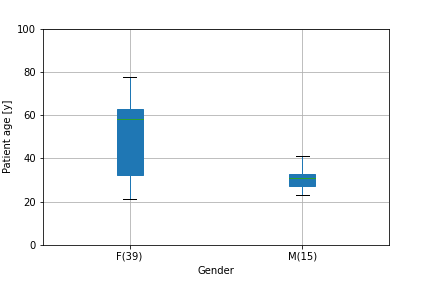
\includegraphics[width=5cm]{automated_graphs/OSF_ageboxplot.png}
        \captionof{figure}{Distribution of patient age in the dataset from the MyoSegmenTUM project.}
        \label{fig:OSF_ageboxplot}
    }


\subsubsection{Technical information}

As shown in figure \ref{fig:OSF_02}, coupes from the second volume of the MyoSegmenTUM dataset are shown.
As is also indicated in figure \ref{fig:AllDataset_dims}, the dimensions of the MyoSegmenTUM volumes is consistent $220 mm \times 220 mm \times 80 mm$, where the shortest dimension is the cropped left-right axis.
There are only three volumes that deviate slightly from this.

\begin{SCfigure}[][htb]
    \centering
    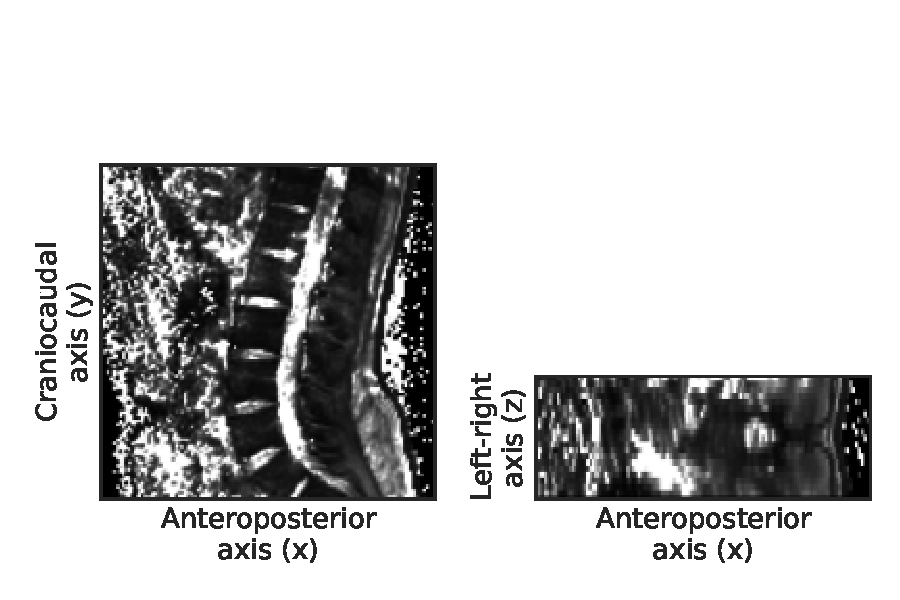
\includegraphics[width=.95\textwidth]{automated_graphs/OSF_02.pdf}
    \caption{MyoSegmenTUM dataset scan \textit{02}. 
    The volumes are cropped in the left-right direction. 
    \label{fig:OSF_02}}
\end{SCfigure}

\begin{SCfigure}[][htb]
    \centering
    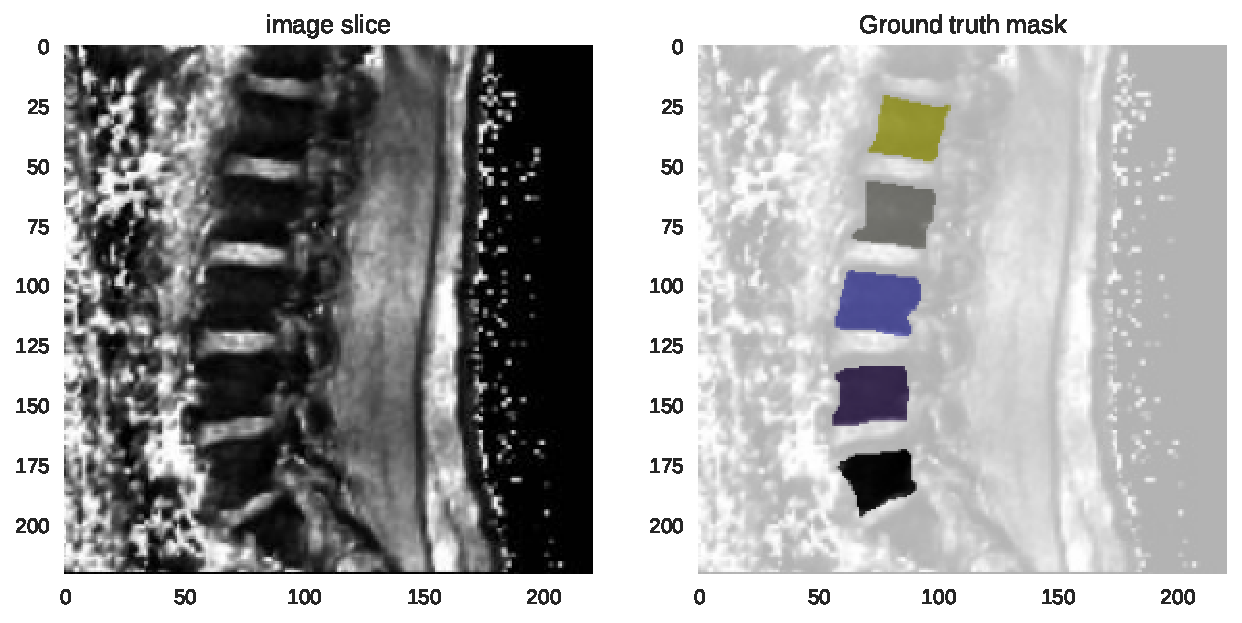
\includegraphics[width=.95\textwidth]{images/MyoSegmenTUM020_s21_mask.pdf}
    \caption{The sagittal slice of MyoSegmenTUM volume 20 is compared to the \Gls{groundtruth} mask.
    For this dataset, only the vertebra body is included in the mask. 
    \protect\newline\noindent Colour legend: \newline
\noindent\mycircle{colL1}  L1 %\newline 
\hspace{2mm}\mycircle{colL2}  L2 %\newline 
\hspace{2mm}\mycircle{colL3}  L3 %\newline 
\hspace{2mm}\mycircle{colL4}  L4 %\newline 
\hspace{2mm}\mycircle{colL5}  L5
    }
\end{SCfigure}

\textbf{Remark:} For three volumes (nr 33, 53 and 54) for which the dimension of the image volume and the label mask do not correspond. 
It is not clear how these masks should be used. 
These volumes were discarded, bringing the final number of volumes used from the MyoSegmenTUM dataset to 51.